% CREATED BY MAGNUS GUSTAVER, 2020
\chapter{Methods}
% All methods used:
% Download Data: 
% - bash: ena browser
% Pipeline 1:
% Annotation Pipeline:
% - TrimGalore! - Trims
%   - MultiQC - Generates a report of the trim-results (it's own pipeline but eh)
% - MetaxaQR - Annotation? SSU/LSU
%   - MetaxaQR_ttt - Taxonomic traversal tool - outputs number of identified SSU/LSU sequences associated with eac node in the taxonomic tree, at different levels (roughly corresponding to kingdoms, phyla, classes, orders, families, genera, species, subspecies, et.c. (We only use first six, down to ~Genus).
%   - MetaxaQR_dc - Data Collector - merges the output of several *.level_X.txt files from _ttt into one large abundance matrix.
% - Diamond - Not used?
%   - Gene Normalization - Not used?
% Create_DB Pipeline:
% - Build_resfinder_db: Only used for Diamond?
% - Build_mobileOG_db: Only used for Diamond?
% 
% Stuff done: 
% - TrimGalore! - Trims - version v0.12.2
%   trim_galore --paired -e 0.1 -j ${task.cpus} --phred33 -q 28 --fastqc ${reads[0]} ${reads[1]}
%   - MultiQC - Generates a report of the trim-results (it's own pipeline but eh) - version 1.18 
%     multiqc -f ${params.trimgalore_path}*fastqc.zip
% - MetaxaQR - Annotation? SSU/LSU - version 3.0 b3
%   metaxaQR -1 read_R1.fastq -2 read_R2.fastq -o ${sample_id}_${params.run_id} --cpu ${task.cpus} -g SSU -d /MetaxaQR/metaxaQR_db/SSU/mqr
%   - MetaxaQR_ttt - Taxonomic traversal tool - outputs number of identified SSU/LSU sequences associated with eac node in the taxonomic tree, at different levels (roughly corresponding to kingdoms, phyla, classes, orders, families, genera, species, subspecies, et.c. (We only use first six, down to ~Genus).
%    metaxaQR_ttt -i ${genus_files} -o ${sample_id}_${params.run_id}  -m 6
%   - MetaxaQR_dc - Data Collector - merges the output of several *.level_X.txt files from _ttt into one large abundance matrix.
%     metaxaQR_dc *.level_6.txt
%
% LaTeX:
% - Boxplots
% - Wilcoxon test
% - Microeco
%   - LEfSe - Not used?
%   - RandomForest

% Other things to mention in method
% - Where data is from
% - CARD
% - Number of samples of each type

% VERSION AV PROGRAMMET BROR, se ovan
% Options? in brackets?

\section{Data Processing}
The data included in this study was downloaded from the European Nucleotide Archive (ENA) at EMBL-EBI\cite{embl-ebi2025ENABrowser}. The full list 16 studies are listed in Appendix \ref{appendix:studies}. 
All except one study were published in the last four years.
In each study only the data from metagenomic analyses was included, the full list of samples may be found in appendix \ref{appendix:samples}. \todo{Where studies found + search terms?} %   à la Goswami}

A total of 395 samples from 53 different locations were analyzed in this study, where figure \ref{world_map} show the location of the samples. 
The samples originate from the Pacific Ocean, along the east coast of the United States, in Europe, Australia, Japan, and China.
These studies were included since they analysed the metagenome in plastic and water substrates, and have published their data in the ENA. Some of them studied non-plastic substrates, however this was not a requirement for inclusion. Studies analysing wastewater were included in order to include samples which should be distinctly different from the water samples, since previous studies have shown that wastewater contributes to antimicrobial resistance \cite{sambaza2023ContributionWastewaterAntimicrobial}.\todo{Mention how the data is aquired in the studies? Throw plastic in ocean -> come back later and collect it -> sequence organisms from surface}

%\todo{M: Explain why these studies were kept for analyses. Think about the substrates and explain your reasonings.}
%\todo{mention that collected data from various ecosystems, which all had different substrates.}

\begin{figure}[h]
    \centering
    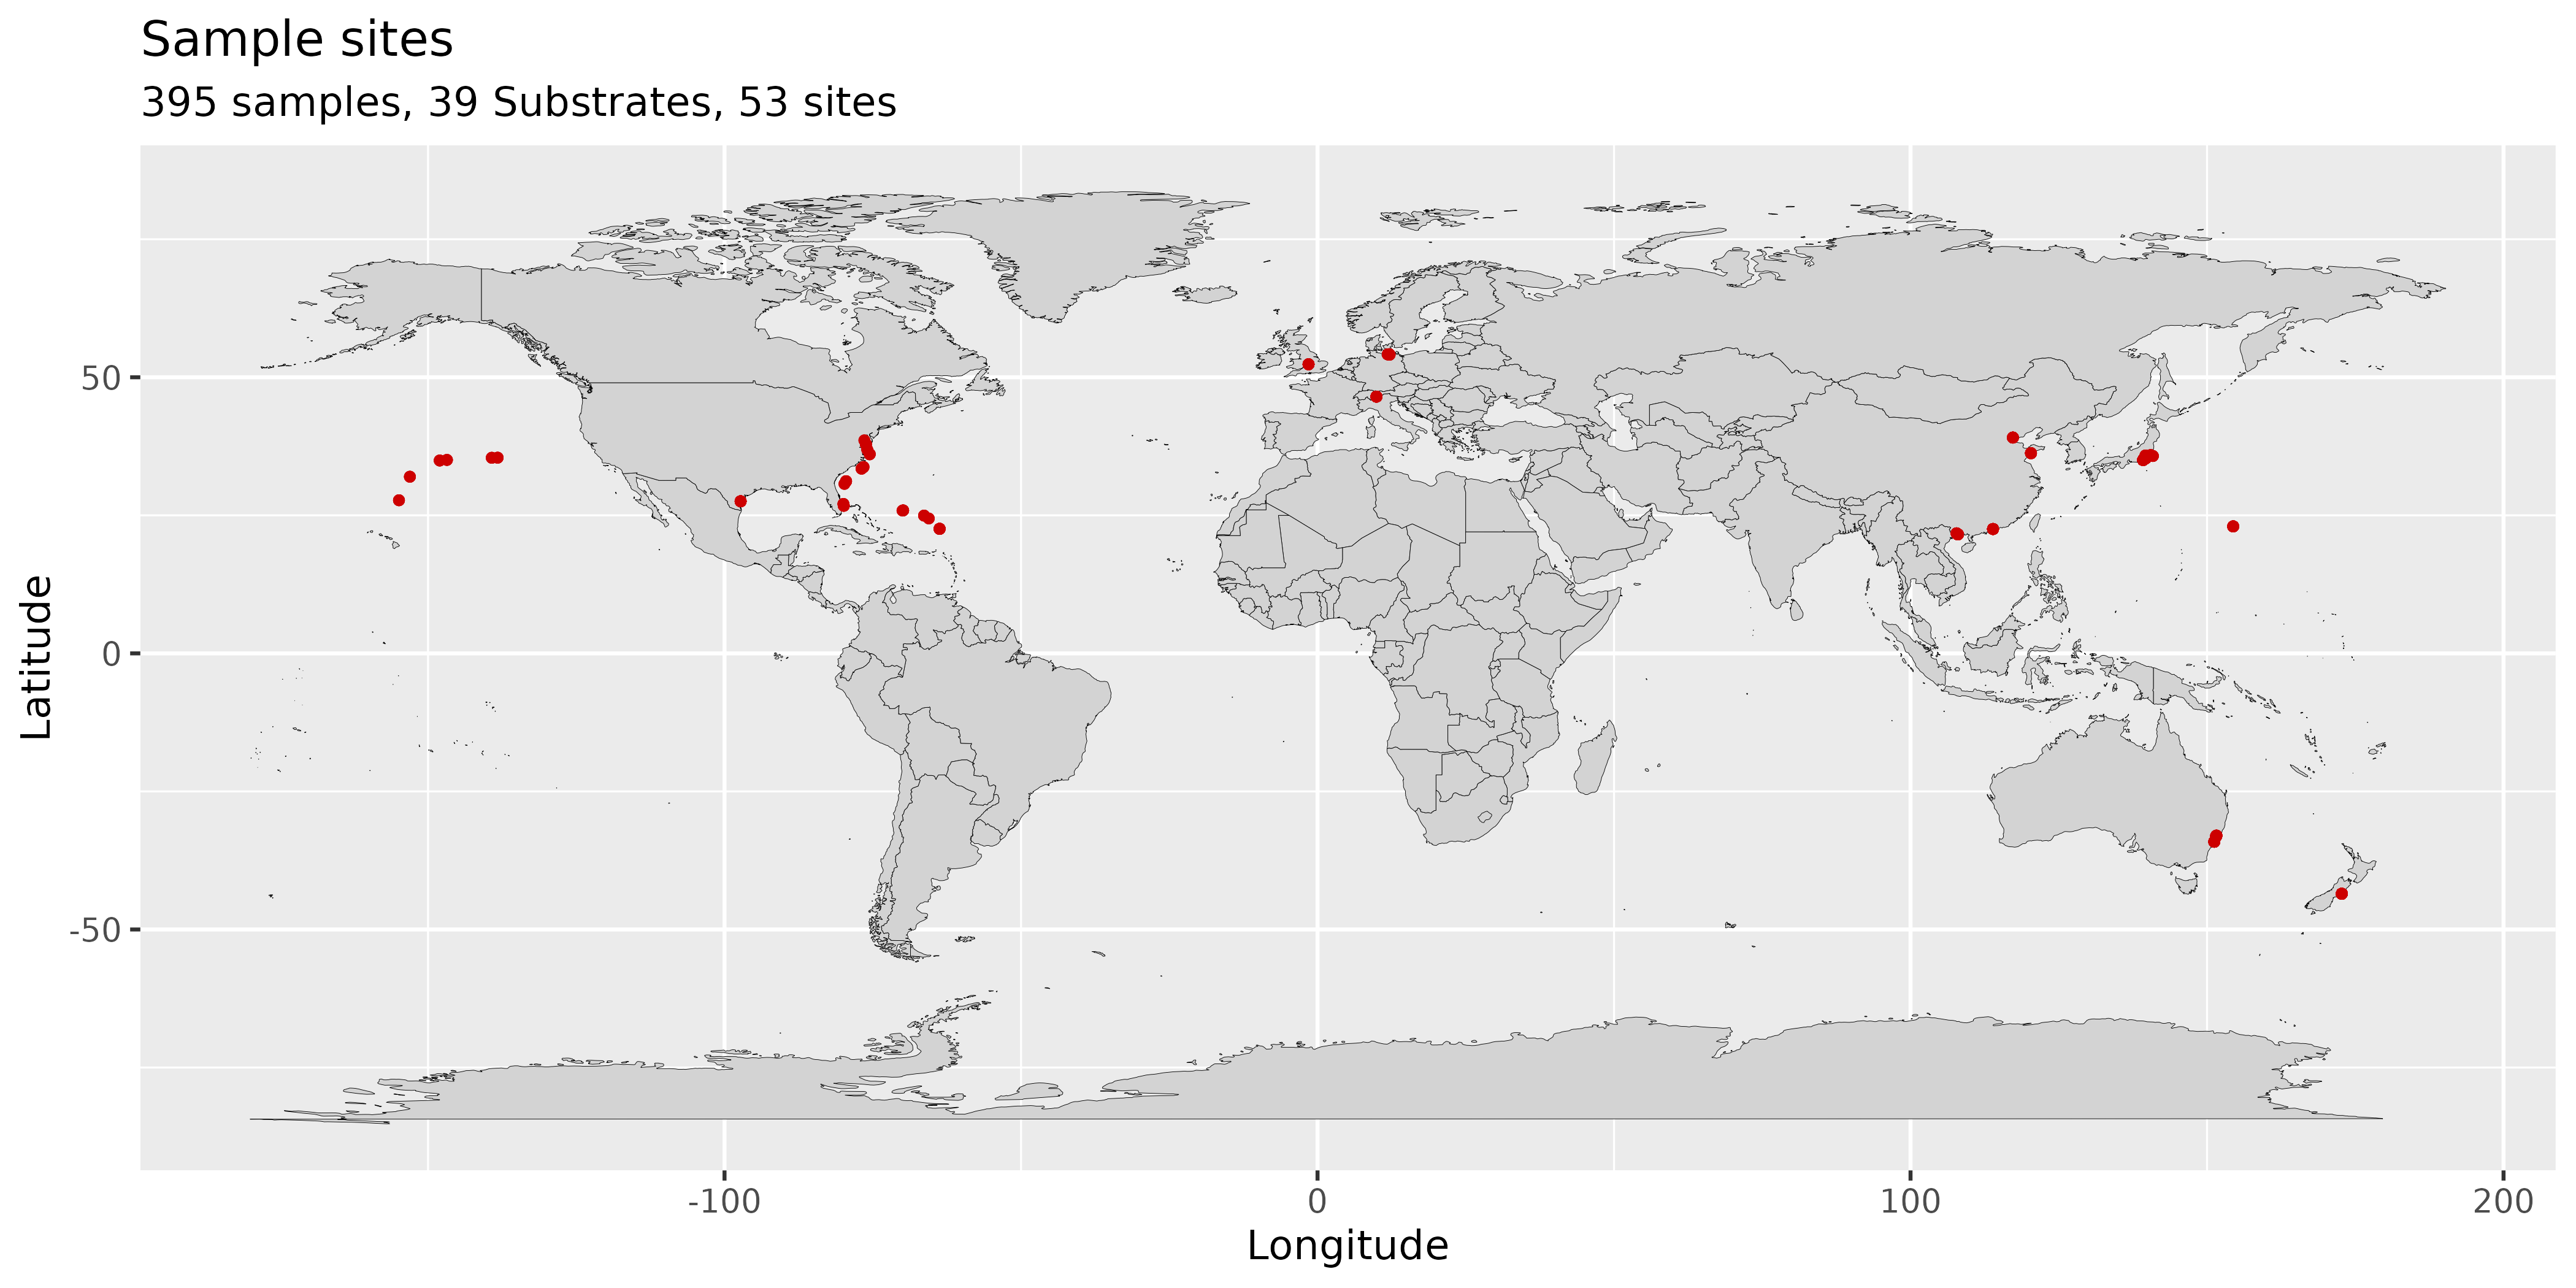
\includegraphics[width = \textwidth]{figure/map.png}
    \caption{Map showing the location of all samples in red}
    \label{world_map}
\end{figure}

The samples were divided into three groups, based on their substrate type as shown in table \ref{substrate_sampletype}. 
The water group included freshwater, seawater, and wastewater samples, the plastic group included 25 different plastics, and the non-plastic group consisted of seven different substrates, such as glass, wood, and soil. 
Each sample was also assigned an ecosystem type of either Ocean, Brackish, River, Wastewater, or Soil, based on the reported sample location.

% \todo{M: this is just one part. Add also that this pipeline was used in order to get taxonomic information as well:} 

An in-house pipeline \cite{wenne2025Pipeline1} was used to trim and filter the data to remove low-quality reads, as well as annotate and map the sequences to databases in order to obtain taxonomic information about the samples.
%In order to trim the reads, filter the data to remove low-quality reads as well as annotate the genomes, an in house pipeline was used\cite{wenne2025Pipeline1}.
To filter the reads TrimGalore (v.0.12.2) \cite{krueger2023TrimGalore0122} was used, which does adapter and quality trimming. It uses FastQC for the quality filtering and Cutadapt for the adapter removal.
The result of the trimming was checked by visualizing the output of the trimming and filtering step using MultiQC\cite{ewels2016MultiQCSummarizeAnalysis}, which outputs an html file containing summarized results for all the samples. 

% --paired - performs length trimming of quality/adaper trimmed reads for paired-end files. 
           % To pass the validation test, both sequences of a pair are required to have minimum length defined.
% -e 0.1 - error rate of 0.1, number of errors divided by length of matching region. DEFAULT
% --phred33 - uses ASCII+33 quality scores as phred scores. DEFAULT
% -q 28 - Trim low-quality ends from reads in addition to adapter removal. Minimum quality of 28.
% --fastqc - Run fastQC in default mode on the fastq file once trimming is done.

After the trimming and filtering step, the remaining reads were annotated using MetaxaQR (v. 3.0 b3)\cite{bengtsson-palme2015Metaxa2Improved}. This tool screens the input sequences for conserved regions of the SSU/LSU gene using hidden Markov models. These models are based on rRNA sequences from the SILVA database\cite{quast2012SILVARibosomalRNA} \todo{skip HMM?}.
    A search using vmatch\cite{kurtzVmatchLargeScale} is then done on the sequences which are found to contain rRNA genes, against a specialized database crafted by the creators of MetaxaQR from release 138 of the SILVA database\cite{bengtsson-palmeMetaxaQRFAQMicrobiologyse}.% and release ten of Mitozoa\cite{donoriodemeo2012MitoZoa20Database}.
The taxonomic annotations are then collected by MetaxaQR Taxonomic Traversal Tool and MetaxaQR Data Collector, which finally outputs one large abundance matrix containing the results from all samples down to the genus level. 

In order to idenify the point mutations present in the samples, the tool MuMaMe (v. 1.0b)\cite{magesh2019MumameSoftwareTool} was used. MuMaMe consists of two tools, MuMaMe\_build and MuMaMe. 
The first tool builds a database of point mutations based on the Comprehensive Antibiotic Resistance Database (CARD) \cite{alcock2023CARD2023Expanded}. In this study the latest version (4.0.0) of CARD was used, which was released in December of 2024.
MuMaMe\_build uses a FASTA sequence file (protein\_fasta\_protein\_variant\_model.fasta) and a list of mutations (snps.txt) to extract sequence excerpts from the FASTA file. It creates one wildtype version and at least one mutated version of the sequence, where if there are several possible mutations close to each other it creates every possible combination of these mutations in addition to the wildtype version. 
The default value, which was used, is to extract 20 residues upstream and downstream of the mutation. 
A maximum depth of 16 was used instead of the default 12. This value limits the maximum amount of mutations that are combined to create the database entries, 
meaning that if there are sufficiently many mutations close to each other not all possible combinations of these will be included in the databasee.

MuMaMe uses the database created by MuMaMe\_build and a FASTQ file, which in this study was the trimmed, filtered and validated files from TrimGalore. MuMaMe auto-detects the other file of the paired-end read and uses both at the same time. It uses usearch\cite{edgar2010SearchClusteringOrders} to map each sequence in the input files to a sequence in the database. Using a best-hit strategy, it can assign the read to either a wildtype sequence or a mutated sequence with higher certainty, since the entries in the database it built will contain both versions of every sequence. \todo{"can map to exactly one of them"?}
MuMaMe outputs a matrix with the number of reads mapped to the mutated and wildtype version of each point mutation, from each sample.
%This file was then used in further analysis in a Jupyter Notebook, available on \href{to do? add link to notebook}{GitHub} 

%\section{Jupyter Notebook}
% In the jupyter notebook, additional files will be used in combination with the results from MuMaMe. These include snps.txt and aro-index.tsv from the CARD\{weird}, as well as a tsv-file containing metadata for all the samples. The first two will be used to label the point mutations with their corresponding resistance mechanism, drug class and AMR gene family, while the last will be used to label the samples.
% 
% The CARD contain some duplicates, which come from different sources. We are not interested in this distinction so only the first one is kept. 

% Additionally, CARD contain some mis-labellings, which mean that some mutation positions seem to be written to occur outside the gene region.
% This issue stems from that the wrong sequence was added to the database in one case and that the original publication of the other mutations published nucleotide substitutions, which got mistaken for amino acid substitutions.
% The curators of the database are aware of this issue\cite{alcockLengthDiscrepancyProtein}.
% MuMaMe is unable to handle these erroneous positions and discards them.
% 
% Some mutations can't be labelled by the metadata, since they are not present in CARD in the unique combination which was found in the sample. 
% For example, if the mutations A12D and Y16S are present in CARD individually, but the combination of them was found in a sample. In these cases the metadata for another mutation in the same gene was used, which may be justified by them sharing the same accession number in the database. \todo{Förklara bättre? Att det är andra mutationer i samma gen som har samma accession?}
% \todo{Göra något med accession = 1, eller bara skippa det?}
% For example, if the above mutations are marked as being mutations in "Mycobacterium tuberculosis embC mutant conferring resistance to ethambutol", they get the same accession number as the other mutations with the same description. 
% The mutations for which labelling of this kind was done, was later assigned an accession number of 1 instead of their usual accesssion number, in order to be identified, but otherwise not disturb the analysis. 
%todo{En mutation utan någon annan liknande? Oklart var den fanns, hitta den? Tror löst?}

%todo{MOVE BOXPLOTS in code to above randomForest?}

\section{Statistical analysis}

The statistical analyses, except the analysis of the number of reads mapped to the point mutations, are based on the relative mutation frequency, where the number of reads matched to the mutated version of the gene is divided by the number of matches to the wildtype version.
Since MuMaMe gives you both values you can use this value instead of scaling the mapped reads to the total read count. 
%This gives you number between zero and one, which signifies how present the mutation is in the sample.

The following analyses will also use the mean mutation percentage, for either the samples or point mutations, which are calculated by grouping the relative mutation frequency by the sample type or substrate, and then by either the sample name or the point mutation identifier. 
A mean is then calculated for each such group, where an example result is shown in table \ref{example_mean_table}.\todo{Should the example be included?} This table shows the relative mutation frequency for two samples, X and Y, for two different mutations, A and B. 
The mean mutation percentage of the two samples are different, 3\% and 11\%, while the mean mutation percentage for the mutations are the same, 7\%.
The mean mutation percentage of the samples estimates "how much mutation has \todo{How can I say this in a more proper way? How large the mean mutation rate of the genes in the samples are?}
occured in the sample". 
On the other hand, the mean mutation percentage for the mutations gives an estimate for how large the mutation rate for specific mutations are in different substrates.
% From results:
% This gives you different results, where in the first case it estimates how mutated the genes are in the samples, i.e. "this sample has a mean mutation percentage of 3\%"
% In the latter case how mutated specific genes are in different substrates, i.e. "mutation A has a mean mutation percentage of 25\% in freshwater".


\begin{table}[h]
    \caption{Example of the calculation of the mean mutation percentage for the samples and mutations respectively}
    \label{example_mean_table}
\begin{tabular}{@{}lll|l@{}}
\toprule
               & Mutation A & Mutation B & Mean samples \\ \midrule
Sample X       & 0.02       & 0.04       & 0.03         \\
Sample Y       & 0.12       & 0.10       & 0.11         \\ \midrule
Mean mutations & 0.07       & 0.07       &              \\ 
\bottomrule 
\end{tabular}
\end{table}

\section{Wilcoxon test}
\todo{Too much? It just happened happened, force of habit I guess}
The statistical analysis of the mean mutation percentage uses the Wilcoxon signed-rank test between the mean mutation percentages for the mutations, and the Wilcoxon rank-sum test between the mean mutation percentage of the samples. 
This difference comes from the fact the genes may be considered paired since they have a data point in each sample, which may be zero, while the samples cannot be paired since there are differing number of samples in each substrate type.

%The Wilcoxon signed-rank test converts the measurement, in our case the mean mutation percentage, to a real number and then calculates the difference between the two paired measurements.
The Wilcoxon signed-rank test calculates the difference between the two paired measurements, in our case the mean mutation percentage, and assigns them a rank based on the absolute value of this difference in ascending order.
The sign of the original difference is kept as the sign of the rank, i.e. if the differences are 5, -7, and 10, the rank numbers are 1, -2, and 3. 
The rank numbers of the two signs are then summed individually. The smaller of these two sums are compared to it's distribution under the null hypothesis, that the distribution is symmetric around $\mu = 0$, from which one then obtains the p-value for the comparison\cite{wilcoxon1945IndividualComparisonsRanking}.

In the analysis, the pseudomean is used to determine the direction of change for the mutation percentage. This pseudomean is not the real pseudomean but instead an estimator for the difference of the location parameters x and y. It estimates the median of the difference between a sample from x and one from y, it does not estimate the difference between the means \cite{thercoreteamWilcoxtestWilcoxonRank}.
% It does not estimate the difference of the means, but instead the median of the difference between a sample from x and a sample from y.

%W = 2
%u = 3 ( 3 + 1 )/ 4 = 3
%s = sqrt( (12*7)/24 ) = 1.87
% --> p-value of 0.6

For the Wilcoxon rank-sum test, the ranks are instead assigned to the values themselves, with the smallest value being assigned the lowest rank. If there are ties the mean rank value is used. The ranks are then summed individually for the two groups, and the value $U$ is calculated for each group according to equation \eqref{equation:wilcox_ranksum}, where $R_i$ is the rank sum of group $i$, and $n_i$ is the number of observations in group $i$.

\begin{equation}
    \label{equation:wilcox_ranksum}
    U_i = R_i - \frac{n_i \left( n_i + 1 \right)}{2}
\end{equation}
The smaller of these values of $U_i$ is then used to get the p-value from the significance table. 

\section{Random Forest}
The random forest method of the differential abundance test (trans\_diff) in the microeco package\cite{liu2021MicroecoPackageData} was used to identify which features are the most important in detemining which sampletype or substrate a sample was from. 
The features used were either AMR Gene Family \todo{explain the AMR Gene Families CARD assigns to mutations here or when first mentioned above? See also theory chapter for explanation.} or the name of the point mutation. 
First a differential test is used to identify significant features, which is then used as input to the random forest algorithm. The random forest algorithm is bootstrapped, repeated, 999 times in order to raise the certainty of the result. 
The random forest algorithm randomly samples a subset of the data, and grows a number of "trees" from it. 
Each tree begin as a single group which is then split in two by randomly selecting a number of features and using the one which achieve the largest decrease in Gini impurity. 
Gini impurity is a meausure of how pure a group is, how close the group is to being of only one class, which would have Gini impurity of zero\cite{ClassificationTreeBinaryDecision}. 
This splitting of the groups is repeated until the tree is complete. 
After all the trees have been grown, the Mean Decrease in Gini Impurity is calculated as the mean of the decrease in Gini impurity for each feature.
It is important to note that a high mean decrease in Gini impurity does not signify that the feature identified is a good classifier for a group has a higher abundance in the group, just that it may be used to identify the group. 















